\section{Procedimento de definição da arquitetura do sistema}

A definição da arquitetura do sistema foi conduzida a partir da combinação entre levantamento bibliográfico, análise técnica das tecnologias envolvidas e separação em módulos da solução proposta. O objetivo dessa etapa foi estruturar uma arquitetura coerente com o problema estudado, considerando as restrições típicas de sistemas embarcados, a necessidade de comunicação em campo e a integração posterior com mecanismos de segurança e análise.

Como referência metodológica para essa definição, o trabalho adota princípios inspirados no modelo RM-ODP, utilizando diferentes pontos de vista para organizar a solução. Em termos funcionais, foram identificados os principais blocos responsáveis pela coleta, encaminhamento, recebimento e armazenamento das informações. Em termos de informação, foram considerados os dados de aplicação e os metadados necessários para rastreabilidade, segurança e análise posterior. Em termos de engenharia, foram observadas as separações entre o trecho embarcado da comunicação, o gateway e a infraestrutura de backend.

A partir dessa organização, a arquitetura foi estruturada de modo a separar claramente a comunicação em campo da camada de aplicação. Essa separação permite tratar, de forma independente, as restrições energéticas dos nós sensores, o papel intermediário do gateway e as funções de autenticação, persistência e análise associadas ao backend. Com isso, a definição arquitetural deixa de ser apenas uma escolha de componentes e passa a refletir a distribuição de responsabilidades entre as partes do sistema.

Além da decomposição dos componentes, o procedimento de definição da arquitetura também considerou o fluxo das informações ao longo da solução. Para isso, foram analisadas as interações entre os nós de campo, o gateway e a infraestrutura de backend, buscando garantir que o sistema fosse capaz de receber, registrar e armazenar dados e metadados de forma compatível com as etapas posteriores do trabalho.

Por fim, a representação da interação entre os principais componentes foi organizada também por meio de diagramas, de modo a tornar mais clara a sequência de eventos envolvida na coleta, no encaminhamento e no armazenamento das mensagens. Essa modelagem auxilia tanto na compreensão da proposta quanto na transição entre a etapa metodológica e a etapa posterior de especificação da arquitetura.

\subsection{Critérios adotados na decomposição arquitetural}

A modularização da arquitetura foi orientada por três critérios principais. O primeiro foi a separação entre o trecho de comunicação em campo e a infraestrutura de aplicação, de modo a preservar as vantagens do uso de LoRa no nível embarcado e da comunicação baseada em rede IP no nível de backend. O segundo foi a definição de responsabilidades distintas para coleta, encaminhamento, autenticação e persistência, evitando concentrar funções heterogêneas em um único componente. O terceiro foi a necessidade de manter a solução compatível com a incorporação posterior de mecanismos de criptografia leve e análise por aprendizado de máquina.

Esses critérios levaram à definição de uma arquitetura em blocos com papéis bem delimitados. No trecho embarcado, concentram-se as funções de aquisição e transmissão inicial dos dados. No ponto de transição, o gateway atua como elemento de integração entre a rede de campo e a infraestrutura de aplicação. No backend, concentram-se as funções de autenticação, persistência e preparação dos dados para uso posterior. Essa divisão favorece clareza arquitetural, reduz acoplamento entre responsabilidades e facilita a evolução incremental da solução.

\subsection{Modelagem das interações e do fluxo de dados}

Para explicitar a dinâmica de funcionamento da proposta, o fluxo principal de interação entre os componentes foi modelado em termos de sequência de eventos. Essa modelagem considera a coleta dos dados no nó de campo, a transmissão pelo enlace LoRa ponto a ponto, a recepção e o enriquecimento da mensagem no gateway, o encaminhamento ao backend por Wi-Fi e HTTP, e o armazenamento final de dados e metadados na infraestrutura de persistência.

A utilização de um diagrama de sequência nessa etapa é importante porque permite representar, de forma mais direta, a ordem das interações entre os componentes e os pontos em que ocorre o tratamento das mensagens. Com isso, o fluxo deixa de ser apenas uma descrição textual e passa a ser apresentado também como uma sequência organizada de ações entre entidades bem definidas.

\begin{figure}[htb]
  \caption{\label{infra_arch_1}Diagrama de sequência UML do fluxo principal}
  \begin{center}
      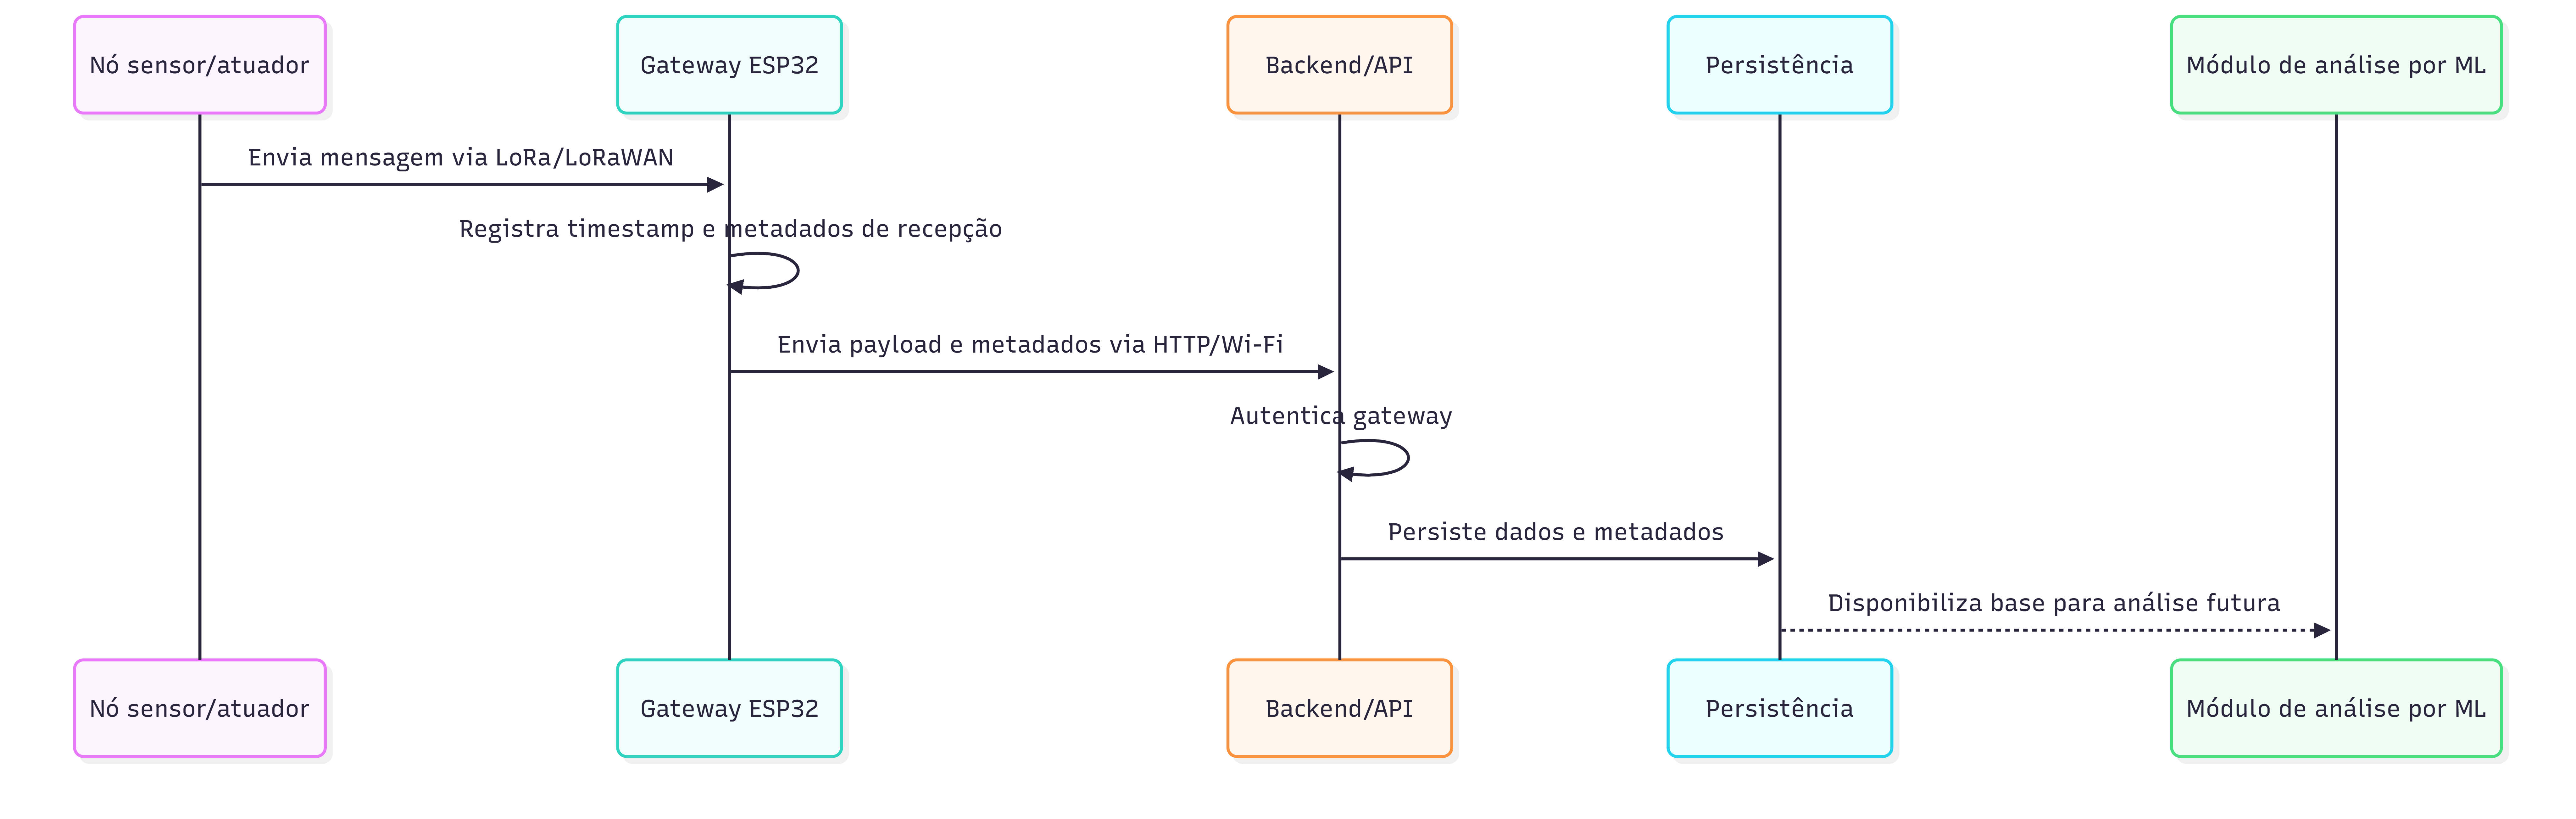
\includegraphics[scale=0.05]{barea/figuras/arch-2-uml.png}
  \end{center}

\end{figure}

Essa representação também ajuda a evidenciar que o sistema foi concebido para operar de forma orientada a evento. Em vez de depender de comunicação contínua, o fluxo é ativado pela geração e recepção das mensagens produzidas em campo, o que torna a proposta mais compatível com o tipo de aplicação e com as restrições energéticas associadas aos dispositivos embarcados.

%%%%%%%%%%%%%%%%%%%%%%%%%%%%%%%%%%%%%%%%%%%%%%%%%%%%
%%%%%%%%%%%%%%%%%%%%%%%%%%%%%%%%%%%%%%%%%%%%%%%%%%%%
